\subsection{Proyección de ventas}

En este apartado se permite realizar un análisis con fines de proyección de resultados financieros futuros de la empresa, de manera que, se pueda observar como el producto se va desenvolver dentro del mercado y anticipa las utilidades y/o perdidas que puedan existir, con el fin de encontrar áreas de oportunidad, fallo, mejora etc. En la tabla \ref{proyeccion} se da una proyección promedio de ventas por mes para cada uno de los planes ofrecidos que consecuentemente genera unos ingresos específicos.

\vspace{2mm}
\begin{minipage}{0.9\textwidth}
\centering
\captionof{table}[{Proyección ventas}]{ Proyección ventas. }
\label{proyeccion}
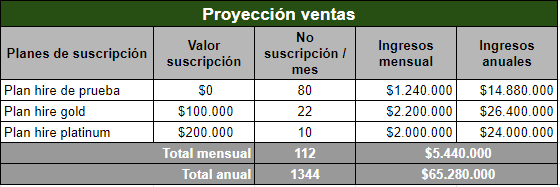
\includegraphics[width=0.9\textwidth]{Images/proyeccionVentas2.png}
\fnote{Nota. \textup{Fuente : Autores}}
\end{minipage}

La proyección considera el IPC propuesto por el equipo técnico del Banco de la República, de forma que, se tenga en cuenta la inflación que pueda existir y las condiciones de posicionamiento de mercado y marketing. A continuación en la tabla \ref{ipc} se indexa la información mencionada.

\vspace{2mm}
\begin{minipage}{0.9\textwidth}
\centering
\captionof{table}[{IPC}]{ IPC. }
\label{ipc}
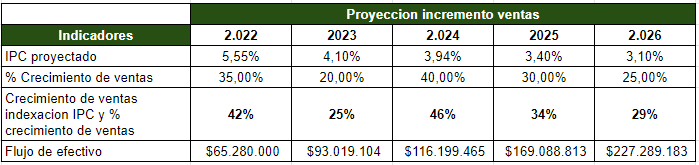
\includegraphics[width=0.9\textwidth]{Images/IPC.png}
\fnote{Nota. \textup{Fuente : Autores}}
\end{minipage}